% =====================================================================
\chapter{Tổng quan về bài báo}
\label{chap:baibao}
% =====================================================================

\section{Mô tả bài báo}

Bài báo được chọn làm đề tài là \emph{``\BaiBaoGoc''} của Snehal Dipak Raut, Sunita P. Ugale và
Dinesh M. Chandwadkar, công bố tại hội nghị ICITSC 2025 \cite{raut2026hybrid}. Thông tin chính của
bài báo được tóm tắt trong \bang{tab:paper-info}.

\begin{table}[H]
\centering
\caption{Thông tin bài báo được tái hiện}
\label{tab:paper-info}
\small
\begin{tabularx}{\linewidth}{@{}P{3.6cm}L@{}}
\toprule
\thead{Mục} & \thead{Nội dung}\\
\midrule
Tên bài báo & \BaiBaoGoc\\
Tác giả & S.\,D.~Raut, S.\,P.~Ugale, D.\,M.~Chandwadkar (K.\,K.~Wagh Institute of Engineering Education and Research, Nashik, Ấn Độ)\\
Nơi công bố & ICITSC 2025 (FusionX Global), Tập 2, tr. 175--182, SCITEPRESS, 2026\\
DOI & 10.5220/0014598700004852\\
Từ khóa & 3DES, AES, Chaos Encryption, Data Security, LSB Steganography\\
Công cụ cài đặt & MATLAB R2024a\\
Dữ liệu thực nghiệm & Linnaeus 5 -- 8000 ảnh màu $256\times256$, 5 lớp \cite{chaladze2017}\\
\bottomrule
\end{tabularx}
\end{table}

Bài toán mà bài báo hướng đến là \textbf{truyền ảnh an toàn qua mạng không tin cậy}, nơi dữ
liệu có thể bị nghe lén, chặn bắt hoặc sửa đổi (chẳng hạn bởi tấn công người đứng giữa -- MITM).
Các tác giả nhận định rằng chỉ mã hóa thì bản mã trông như nhiễu và dễ thu hút sự chú ý, còn chỉ
giấu tin thì nội dung sẽ lộ ngay khi bị phát hiện. Từ đó bài báo đề xuất một \textbf{khung lai
mật mã -- giấu tin} hai lớp: ảnh bí mật được mã hóa bằng một trong ba thuật toán (\textbf{3DES},
\textbf{AES} hoặc \textbf{mã hóa hỗn loạn kết hợp mặt nạ giả ngẫu nhiên}), sau đó bản mã được
nhúng vào 1--3 bit thấp của một ảnh phủ màu $256\times256$.

Đóng góp chính của bài báo gồm:
\begin{itemize}
  \item Xây dựng ba biến thể của cùng một khung: \textbf{3DES-LSB}, \textbf{AES-LSB} và
        \textbf{Chaotic + PRNG Masking LSB};
  \item Đánh giá trên toàn bộ 8000 ảnh của Linnaeus 5 bằng một bộ độ đo gồm chất lượng thị giác
        (MSE, PSNR, SSIM), độ an toàn thống kê (NPCR, UACI, entropy, hệ số tương quan) và tốc độ
        mã hóa;
  \item Đưa ra khuyến nghị: phương pháp hỗn loạn nhanh hơn khoảng hai bậc độ lớn nên phù hợp
        ứng dụng thời gian thực, còn AES/3DES phù hợp với các hệ thống cần tuân thủ chuẩn mật mã.
\end{itemize}

\section{Vấn đề và giải pháp liên quan đến bài toán}

\subsection{Kiến thức cơ sở}

\subsubsection{DES và Triple DES (3DES)}

DES (\tn{Data Encryption Standard}) là mã khối cấu trúc Feistel 16 vòng, khối 64 bit, khóa
56 bit hiệu dụng (64 bit kể cả 8 bit chẵn lẻ). Với sức mạnh tính toán hiện nay, khóa 56 bit
có thể bị vét cạn nên DES không còn an toàn. \textbf{Triple DES} (3DES, hay TDEA) kéo dài tuổi
thọ của DES bằng cách áp dụng DES ba lần theo trình tự \textbf{mã hóa -- giải mã -- mã hóa}
(EDE) với ba khóa con $K_1, K_2, K_3$ \cite{sp80067}:
\begin{equation}
  C = E_{K_3}\Bigl(D_{K_2}\bigl(E_{K_1}(P)\bigr)\Bigr), \qquad
  P = D_{K_1}\Bigl(E_{K_2}\bigl(D_{K_3}(C)\bigr)\Bigr).
  \label{eq:3des}
\end{equation}
Với ba khóa độc lập (khóa 192 bit, tức 168 bit hiệu dụng), do tấn công gặp nhau ở giữa
(\tn{meet-in-the-middle}) nên độ an toàn thực tế của 3DES chỉ khoảng 112 bit. Thiết kế EDE còn
bảo đảm tương thích ngược: khi $K_1 = K_2 = K_3$, 3DES suy biến thành DES đơn. Vì kích thước khối
chỉ 64 bit, 3DES dễ bị tấn công va chạm khi mã hóa lượng dữ liệu lớn với cùng một khóa
(tấn công Sweet32 \cite{bhargavan2016}). NIST đã không cho phép dùng 3DES để mã hóa dữ liệu mới
sau năm 2023 \cite{sp800131a}.

\begin{figure}[H]
\centering
\begin{tikzpicture}[node distance=7mm]
  \node (p) {$P$ (64 bit)};
  \node[pbox, right=of p] (e1) {$E_{K_1}$\\DES};
  \node[pbox, right=of e1] (d2) {$D_{K_2}$\\DES$^{-1}$};
  \node[pbox, right=of d2] (e3) {$E_{K_3}$\\DES};
  \node[right=of e3] (c) {$C$ (64 bit)};
  \draw[arr] (p) -- (e1); \draw[arr] (e1) -- (d2); \draw[arr] (d2) -- (e3); \draw[arr] (e3) -- (c);
  \node[lbl, below=2mm of d2] {Khóa 192 bit $= K_1 \,\|\, K_2 \,\|\, K_3$ (mỗi khóa 64 bit gồm 56 bit hiệu dụng)};
\end{tikzpicture}
\caption{Cấu trúc mã hóa 3DES theo trình tự EDE}
\label{fig:3des}
\end{figure}

\subsubsection{Chuẩn mã hóa nâng cao AES}

AES (\tn{Advanced Encryption Standard}) được NIST chuẩn hóa năm 2001 để thay thế DES
\cite{fips197, daemen2002}. AES là mạng thay thế -- hoán vị (SPN) làm việc trên khối 128 bit được
biểu diễn thành ma trận trạng thái $4\times4$ byte. Với khóa 128, 192 và 256 bit, số vòng tương ứng
là 10, 12 và 14. Mỗi vòng (trừ vòng cuối không có MixColumns) gồm bốn phép biến đổi:
\begin{itemize}
  \item \textbf{SubBytes}: thay thế từng byte qua hộp S-box phi tuyến xây dựng từ phép nghịch đảo
        trong trường hữu hạn $\mathrm{GF}(2^8)$ kết hợp biến đổi affine, tạo tính \emph{hỗn loạn}
        (\tn{confusion});
  \item \textbf{ShiftRows}: dịch vòng hàng $i$ của ma trận trạng thái sang trái $i$ byte;
  \item \textbf{MixColumns}: nhân mỗi cột với một ma trận cố định trên $\mathrm{GF}(2^8)$, tạo tính
        \emph{khuếch tán} (\tn{diffusion});
  \item \textbf{AddRoundKey}: XOR trạng thái với khóa vòng sinh ra từ thuật toán mở rộng khóa.
\end{itemize}
Đến nay chưa có tấn công thực tế nào làm suy yếu đáng kể AES khi được dùng đúng cách. Các CPU
hiện đại còn có tập lệnh phần cứng AES-NI giúp AES đạt tốc độ rất cao.

\subsubsection{Chế độ CBC và đệm PKCS\#7}

Cả 3DES và AES trong bài báo đều chạy ở \textbf{chế độ CBC} (\tn{Cipher Block Chaining})
\cite{sp80038a}. Bản rõ được chia thành các khối $P_1, \dots, P_n$; mỗi khối được XOR với khối
bản mã trước đó rồi mới đưa vào hàm mã hóa, với khối đầu tiên dùng vectơ khởi tạo IV:
\begin{equation}
  C_0 = \mathit{IV}, \qquad C_i = E_K\left(P_i \xor C_{i-1}\right), \qquad
  P_i = D_K(C_i) \xor C_{i-1}, \quad i = 1, \dots, n.
  \label{eq:cbc}
\end{equation}
Từ \pt{eq:cbc} có thể rút ra hai tính chất sẽ được kiểm chứng ở Chương~\ref{chap:vandung}:
\begin{itemize}
  \item \textbf{Lan truyền khi mã hóa}: thay đổi một bit ở khối $P_i$ làm thay đổi toàn bộ các
        khối $C_i, C_{i+1}, \dots, C_n$, nhưng không ảnh hưởng các khối đứng trước $C_i$;
  \item \textbf{Lan truyền lỗi khi giải mã}: một bit lỗi trong $C_i$ làm hỏng hoàn toàn khối
        $P_i$ và đảo đúng một bit tương ứng trong $P_{i+1}$; các khối khác không bị ảnh hưởng.
\end{itemize}

\begin{figure}[H]
\centering
\begin{tikzpicture}[x=3.4cm, y=1cm]
  \foreach \i/\x in {1/1, 2/2, 3/3}{
    \node (p\i) at (\x, 2.2) {$P_{\i}$};
    \node[xorn] (x\i) at (\x, 1.3) {$\oplus$};
    \node[pbox, minimum width=16mm] (e\i) at (\x, 0.2) {$E_K$};
    \node (c\i) at (\x, -0.9) {$C_{\i}$};
    \draw[arr] (p\i) -- (x\i);
    \draw[arr] (x\i) -- (e\i);
    \draw[arr] (e\i) -- (c\i);
  }
  \node (iv) at (0.2, 1.3) {$\mathit{IV}$};
  \draw[arr] (iv) -- (x1);
  \draw[arr] ($(e1.south)+(0,-0.35)$) -| ++(0.5,0) |- (x2);
  \draw[arr] ($(e2.south)+(0,-0.35)$) -| ++(0.5,0) |- (x3);
\end{tikzpicture}
\caption{Mã hóa ở chế độ CBC}
\label{fig:cbc}
\end{figure}

Vì mã khối chỉ xử lý dữ liệu có độ dài là bội số của kích thước khối $b$ ($b=8$ byte với 3DES,
$b=16$ byte với AES), bản rõ phải được \textbf{đệm} (\tn{padding}). Chuẩn PKCS\#7
\cite{rfc5652} thêm $n = b - (|M| \bmod b)$ byte, mỗi byte có giá trị bằng $n$
($1 \le n \le b$). Ví dụ, với $b = 8$ và bản rõ dài 5 byte thì cần thêm 3 byte
\code{03 03 03}; nếu bản rõ đã đủ bội số của $b$ thì vẫn thêm nguyên một khối gồm $b$ byte
giá trị $b$. Khi giải mã, nếu byte cuối không tạo thành chuỗi đệm hợp lệ thì phép gỡ đệm báo
lỗi. Tính chất này khiến việc giải mã bằng sai khóa gần như luôn bị phát hiện, vì khối cuối
giải mã ra dữ liệu rác. Ảnh $156\times156$ (\num{24336} byte) sau khi đệm thành \num{24344}
byte với 3DES và \num{24352} byte với AES.

\subsubsection{Hệ hỗn loạn và ánh xạ Logistic}

Hệ hỗn loạn (\tn{chaotic system}) là hệ động lực tất định nhưng có hành vi trông như ngẫu nhiên
và \textbf{cực kỳ nhạy cảm với điều kiện đầu}. Tính chất này giống các yêu cầu hỗn loạn và khuếch
tán của Shannon \cite{shannon1949}, nên hệ hỗn loạn được dùng rộng rãi để thiết kế mã hóa ảnh
\cite{kocarev2001}. Ánh xạ \textbf{Logistic} là một trong những hệ hỗn loạn đơn giản nhất
\cite{may1976}:
\begin{equation}
  x_{n+1} = r \cdot x_n \cdot (1 - x_n), \qquad x_n \in (0, 1),\; r \in (0, 4].
  \label{eq:logistic}
\end{equation}
Khi $r$ tăng từ khoảng $3$ trở lên, hệ trải qua chuỗi rẽ nhánh nhân đôi chu kỳ và bước vào miền
hỗn loạn khi $r \gtrsim 3.57$ (\hinh{fig:logistic}a). Bài báo chọn $x_0 = 0.785398$ và
$r = 3.999$, sát giá trị $4$ để chuỗi phân bố trên gần như toàn bộ khoảng $(0,1)$.
\hinh{fig:logistic}b cho thấy hai quỹ đạo xuất phát từ $x_0$ và $x_0 + 10^{-10}$ trùng nhau ở
khoảng 30 bước đầu rồi tách rời hoàn toàn.

\begin{figure}[H]
\centering
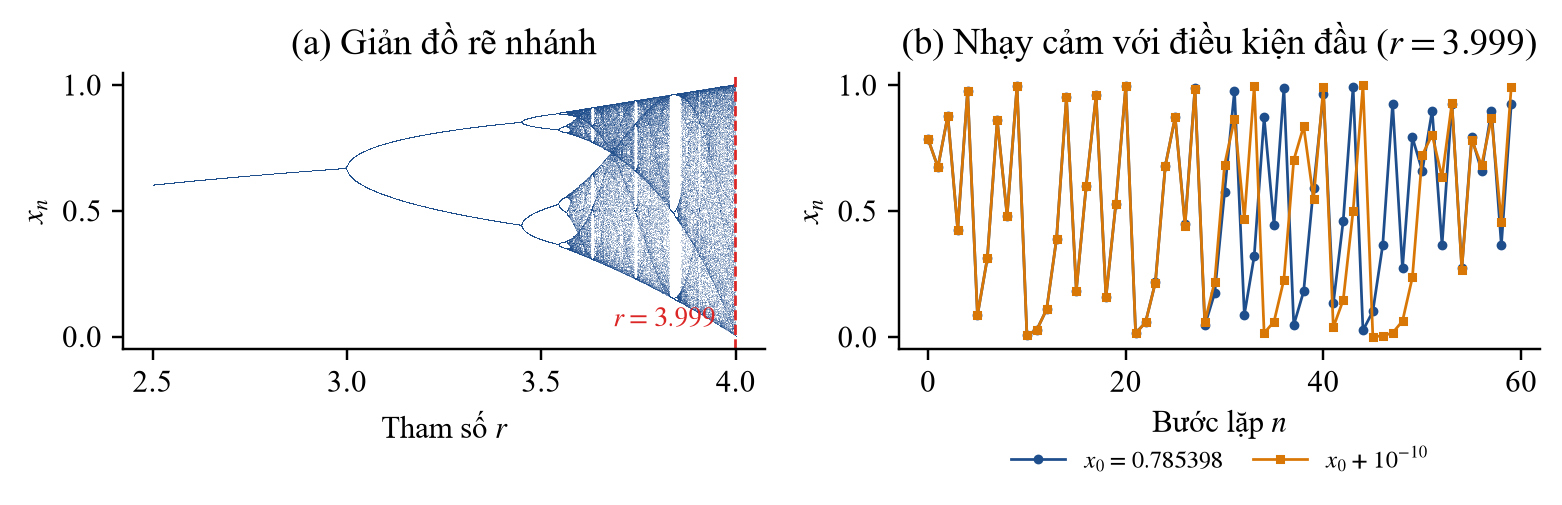
\includegraphics[width=\linewidth]{logistic_map}
\caption{Ánh xạ Logistic: (a) giản đồ rẽ nhánh theo $r$; (b) độ nhạy với điều kiện đầu}
\label{fig:logistic}
\end{figure}

Tuy vậy, cần lưu ý rằng ``hỗn loạn'' không đồng nghĩa với ``an toàn mật mã''. Alvarez và Li
\cite{alvarez2006} chỉ ra nhiều lược đồ mã hóa hỗn loạn bị phá vì không gian khóa nhỏ, phân bố
chuỗi không đều hoặc dùng lại dòng khóa. Đây là cơ sở để đánh giá lớp mã hóa hỗn loạn của bài
báo ở mục~\ref{sec:antoan-morong}.

\subsubsection{Toán tử XOR và mã dòng}

Phép XOR ($\xor$) có các tính chất giao hoán, kết hợp, $A \xor 0 = A$ và tự nghịch đảo
$A \xor A = 0$. Do đó nếu $C = P \xor K$ thì $P = C \xor K$, tức cùng một phép toán được dùng cho
cả mã hóa và giải mã. Khi dòng khóa $K$ thật sự ngẫu nhiên, dài bằng bản rõ và \emph{chỉ dùng một
lần}, ta có sổ mật mã dùng một lần (\tn{one-time pad}), an toàn tuyệt đối theo Shannon
\cite{shannon1949}. Ngược lại, nếu cùng một dòng khóa được dùng cho hai bản rõ $P_1, P_2$ thì:
\begin{equation}
  C_1 \xor C_2 = (P_1 \xor K) \xor (P_2 \xor K) = P_1 \xor P_2,
  \label{eq:twotime}
\end{equation}
nghĩa là dòng khóa bị triệt tiêu và cấu trúc của hai bản rõ lộ ra. Hơn nữa, chỉ cần biết một
cặp $(P_1, C_1)$ là kẻ tấn công khôi phục được $K = P_1 \xor C_1$ \cite{katz2020}.

\subsubsection{Giấu tin LSB đa bit}

Với điểm ảnh 8 bit có giá trị $c$, kỹ thuật \textbf{$k$-LSB} thay $k$ bit thấp nhất của $c$ bằng
một nhóm $k$ bit thông điệp có giá trị $m \in \{0, \dots, 2^k - 1\}$:
\begin{equation}
  s = c - (c \bmod 2^k) + m, \qquad |s - c| \le 2^k - 1.
  \label{eq:klsb}
\end{equation}
Mỗi kênh màu R, G, B được dùng như một ``điểm'' nhúng độc lập nên ảnh màu $H \times W$ có dung
lượng $3HWk$ bit. \hinh{fig:lsb-example} minh họa nhúng 1 bit và 3 bit vào một giá trị kênh màu.

\begin{figure}[H]
\centering
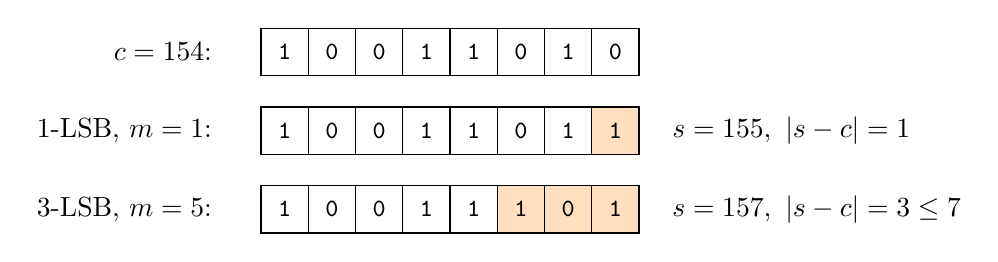
\begin{tikzpicture}[
  bit/.style={draw, minimum width=6mm, minimum height=6mm, font=\ttfamily\small, inner sep=0pt},
  hb/.style={bit, fill=orange!25}]
  \node[anchor=east] at (-0.2, 0) {$c = 154$:};
  \foreach \b [count=\i] in {1,0,0,1,1,0,1,0}{ \node[bit] at (\i*0.6, 0) {\b}; }
  \node[anchor=east] at (-0.2, -1) {1-LSB, $m=1$:};
  \foreach \b [count=\i] in {1,0,0,1,1,0,1}{ \node[bit] at (\i*0.6, -1) {\b}; }
  \node[hb] at (4.8, -1) {1};
  \node[anchor=west] at (5.4, -1) {$s = 155,\ |s-c| = 1$};
  \node[anchor=east] at (-0.2, -2) {3-LSB, $m=5$:};
  \foreach \b [count=\i] in {1,0,0,1,1}{ \node[bit] at (\i*0.6, -2) {\b}; }
  \foreach \b [count=\i] in {1,0,1}{ \node[hb] at (3.0+\i*0.6, -2) {\b}; }
  \node[anchor=west] at (5.4, -2) {$s = 157,\ |s-c| = 3 \le 7$};
\end{tikzpicture}
\caption{Ví dụ nhúng 1-LSB và 3-LSB vào một giá trị kênh màu (ô tô màu là bit thông điệp)}
\label{fig:lsb-example}
\end{figure}

Khi bit thông điệp là ngẫu nhiên đều và độc lập với ảnh phủ (đúng với bản mã tốt), $k$ bit thấp
của $c$ và $m$ đều phân bố đều trên $\{0,\dots,L-1\}$ với $L = 2^k$. Sai số bình phương kỳ vọng
tại mỗi kênh khi đó bằng:
\begin{equation}
  \mathbb{E}\bigl[(s-c)^2\bigr] = 2\,\mathrm{Var}(U_L) = \frac{L^2 - 1}{6}
  = \begin{cases} 0.5 & k = 1,\\ 2.5 & k = 2,\\ 10.5 & k = 3. \end{cases}
  \label{eq:lsb-mse}
\end{equation}
Công thức \pt{eq:lsb-mse} là chìa khóa để giải thích các con số MSE và PSNR trong bài báo:
nhúng 1-LSB lấp đầy toàn bộ ảnh cho $\mathrm{MSE} \approx 0.5$, tương ứng
$\mathrm{PSNR} = 10\log_{10}(255^2/0.5) \approx \SI{51.14}{dB}$.

\subsection{Tiêu chí đánh giá}
\label{sec:tieuchi}

Bài báo dùng ba nhóm tiêu chí: chất lượng thị giác của ảnh mang tin, độ an toàn thống kê của bản
mã và tốc độ thực thi.

\subsubsection{Sai số bình phương trung bình và PSNR}

Với ảnh phủ $I$ và ảnh mang tin $K$ kích thước $M \times N$ (mỗi điểm ảnh có $c$ kênh):
\begin{equation}
  \mathrm{MSE} = \frac{1}{MNc}\sum_{i,j,ch}\bigl[I(i,j,ch) - K(i,j,ch)\bigr]^2, \qquad
  \mathrm{PSNR} = 10\log_{10}\frac{255^2}{\mathrm{MSE}} \;(\mathrm{dB}).
  \label{eq:mse-psnr}
\end{equation}
MSE càng nhỏ và PSNR càng lớn thì ảnh mang tin càng giống ảnh phủ; PSNR trên khoảng
\SI{40}{dB} thường được coi là không phân biệt được bằng mắt thường. Bài báo ghi mẫu số của MSE
là $M \times N$; tuy nhiên để ra được $\mathrm{MSE} \approx 0.5$ như Bảng~2 của bài báo thì phải
chia cho toàn bộ $M \times N \times 3$ phần tử (giống hàm \code{immse} của MATLAB).

\subsubsection{Chỉ số tương đồng cấu trúc SSIM}

SSIM \cite{wang2004ssim} so sánh độ sáng, độ tương phản và cấu trúc cục bộ của hai ảnh $x, y$:
\begin{equation}
  \mathrm{SSIM}(x,y) = \frac{(2\mu_x\mu_y + C_1)(2\sigma_{xy} + C_2)}
                            {(\mu_x^2 + \mu_y^2 + C_1)(\sigma_x^2 + \sigma_y^2 + C_2)},
  \label{eq:ssim}
\end{equation}
trong đó $\mu$, $\sigma^2$, $\sigma_{xy}$ là trung bình, phương sai và hiệp phương sai tính trên cửa
sổ trượt; $C_1 = (0.01\cdot255)^2$, $C_2 = (0.03\cdot255)^2$. SSIM nằm trong $[-1, 1]$ và bằng 1
khi hai ảnh giống hệt nhau.

\subsubsection{Phân tích histogram}

Histogram biểu diễn tần suất xuất hiện của từng mức xám. Ảnh tự nhiên có histogram nhiều đỉnh,
không đều; một thuật toán mã hóa tốt phải cho histogram bản mã gần như \emph{phẳng}, nhờ đó chống
được tấn công thống kê. Ngược lại, histogram của ảnh mang tin phải gần như trùng với histogram ảnh
phủ để không để lại dấu vết.

\subsubsection{Phân tích vi sai: NPCR và UACI}

NPCR (\tn{Number of Pixels Change Rate}) đo tỷ lệ điểm ảnh khác nhau giữa hai ảnh $I_1, I_2$
kích thước $m\times n$; UACI (\tn{Unified Average Changing Intensity}) đo độ chênh cường độ trung
bình \cite{wu2011npcr}:
\begin{equation}
  \mathrm{NPCR} = \frac{1}{mn}\sum_{i,j} D(i,j)\times100\%, \quad
  D(i,j) = \begin{cases}0 & I_1(i,j) = I_2(i,j)\\ 1 & I_1(i,j) \neq I_2(i,j)\end{cases},
  \label{eq:npcr}
\end{equation}
\begin{equation}
  \mathrm{UACI} = \frac{1}{mn}\sum_{i,j}\frac{|I_1(i,j) - I_2(i,j)|}{255}\times100\%.
  \label{eq:uaci}
\end{equation}
Với hai ảnh ngẫu nhiên đều và độc lập, giá trị kỳ vọng là
$\mathrm{NPCR} = (1 - 2^{-8})\times100\% \approx 99.609\%$ và $\mathrm{UACI} \approx 33.464\%$
\cite{wu2011npcr}. Cần lưu ý: theo định nghĩa chuẩn của phân tích vi sai, $I_1$ và $I_2$ là
\emph{hai bản mã} của hai bản rõ chỉ khác nhau một điểm ảnh. Bài báo lại tính NPCR, UACI giữa
\emph{ảnh bí mật và bản mã của chính nó}; khác biệt này được phân tích ở
mục~\ref{sec:antoan-morong}.

\subsubsection{Entropy thông tin}

Entropy Shannon \cite{shannon1948} đo độ bất định trung bình của một điểm ảnh:
\begin{equation}
  H = -\sum_{i=0}^{L-1} p_i \log_2 p_i \quad (\text{bit}),
  \label{eq:entropy}
\end{equation}
với $L = 256$ mức xám và $p_i$ là xác suất xuất hiện mức $i$. Giá trị tối đa là 8 bit, đạt được
khi phân bố đều; bản mã tốt phải có entropy rất gần 8.

\subsubsection{Hệ số tương quan}

Hệ số tương quan Pearson giữa hai dãy giá trị $x, y$ độ dài $N$:
\begin{equation}
  r_{xy} = \frac{\sum_{i=1}^N (x_i - \bar x)(y_i - \bar y)}
                {\sqrt{\sum_{i=1}^N (x_i - \bar x)^2}\sqrt{\sum_{i=1}^N (y_i - \bar y)^2}}.
  \label{eq:corr}
\end{equation}
Bài báo dùng $r$ giữa ảnh bí mật và bản mã (kỳ vọng $r \approx 0$). Một cách dùng phổ biến khác
là tương quan giữa các cặp \emph{điểm ảnh kề nhau} theo chiều ngang, dọc, chéo: ảnh tự nhiên có
$r$ gần 1, bản mã tốt phải có $r$ gần 0.

\subsubsection{Thời gian mã hóa}

Thời gian mã hóa (\tn{EncTime}) đo chi phí tính toán của bước mã hóa ảnh bí mật; giá trị càng nhỏ
thì thuật toán càng phù hợp cho ứng dụng thời gian thực hoặc thiết bị hạn chế tài nguyên.

\subsection{Kỹ thuật áp dụng trong bài báo}

\subsubsection{Kiến trúc tổng thể}

Khung đề xuất gồm hai lớp nối tiếp (\hinh{fig:paper-arch}). Ở phía gửi, ảnh bí mật xám được
chuyển thành chuỗi byte và mã hóa thành ``ảnh mã hóa'' trông như nhiễu; sau đó bản mã được nhúng
vào các bit LSB của ảnh phủ màu để tạo ảnh mang tin. Ở phía nhận, các bit LSB được trích xuất để
dựng lại bản mã và giải mã bằng đúng khóa để thu lại ảnh bí mật.

\begin{figure}[H]
\centering
\resizebox{\linewidth}{!}{%
\begin{tikzpicture}[every node/.append style={font=\footnotesize}]
  \node[box] (si) {Ảnh bí mật\\(xám)};
  \node[pbox, right=8mm of si] (enc) {Mã hóa\\3DES / AES / Chaotic};
  \node[pbox, right=17mm of enc] (st) {Giấu tin\\LSB (1--3 bit)};
  \node[box, above=7mm of st] (cov) {Ảnh phủ\\RGB $256\times256$};
  \node[pbox, right=22mm of st] (dr) {Trích xuất\\và giải mã};
  \node[box, right=8mm of dr] (rs) {Ảnh bí mật\\khôi phục};
  \draw[arr] (si) -- (enc);
  \draw[arr] (enc) -- node[lbl, above] {bản mã} (st);
  \draw[arr] (cov) -- (st);
  \draw[arr] (st) -- node[lbl, above, pos=0.28] {ảnh stego} (dr);
  \draw[arr] (dr) -- (rs);
  \node[lbl, below=2mm of enc] {khóa $K$};
  \node[lbl, below=2mm of dr] {khóa $K$};
  \coordinate (mid) at ($(st.east)!0.6!(dr.west)$);
  \draw[dashed, gray] ($(mid)+(0,0.9)$) -- ($(mid)+(0,-0.8)$);
  \node[lbl, gray, anchor=south] at ($(mid)+(0,0.9)$) {kênh công khai};
\end{tikzpicture}}
\caption{Sơ đồ khối của hệ mật mã -- giấu tin kết hợp (vẽ lại theo Hình~1 của bài báo
\cite{raut2026hybrid})}
\label{fig:paper-arch}
\end{figure}

\subsubsection{Phương pháp 3DES-LSB}

\begin{enumerate}
  \item Chuyển ảnh bí mật thành chuỗi byte; mã hóa bằng 3DES khóa 192 bit (24 byte), IV 64 bit
        (8 byte), chế độ CBC, trình tự EDE.
  \item Xác định số bit LSB cần dùng trên mỗi kênh màu (1--3 bit) từ kích thước bản mã và số điểm
        ảnh của ảnh phủ.
  \item Chuyển bản mã thành chuỗi bit và nhúng vào các bit LSB của ảnh phủ RGB.
  \item Phía nhận trích các bit LSB, dựng lại bản mã, giải mã bằng cùng khóa và IV.
  \item Định hình lại (\tn{reshape}) dữ liệu giải mã về kích thước ban đầu của ảnh bí mật.
  \item Tính các độ đo chất lượng (MSE, PSNR, SSIM) và an toàn (NPCR, UACI, tương quan, entropy).
\end{enumerate}

\subsubsection{Phương pháp AES-LSB}

Quy trình hoàn toàn tương tự 3DES-LSB, chỉ khác lớp mã hóa: AES-128 với khóa 16 byte, IV 16 byte,
chế độ CBC. Kích thước khối 128 bit khiến bản mã được đệm thành bội số của 16 byte.

\subsubsection{Phương pháp Chaotic + PRNG Masking}

Lớp mã hóa thứ ba là một mã dòng gồm hai mặt nạ cùng độ dài $N$ với chuỗi byte ảnh bí mật $S$
(\hinh{fig:paper-chaotic}):
\begin{itemize}
  \item \textbf{Mặt nạ hỗn loạn}: sinh dãy $\{x_n\}$ theo \pt{eq:logistic} với $x_0 = 0.785398$,
        $r = 3.999$, rồi co giãn về khoảng $0$--$255$;
  \item \textbf{Mặt nạ ``ECC'' mô phỏng}: một dãy byte giả ngẫu nhiên sinh từ một hạt giống
        (\tn{seed}) cố định, được tác giả gọi là mô phỏng dòng khóa ECC.
\end{itemize}
Bản mã được tính bằng hai phép XOR liên tiếp, và giải mã chính là lặp lại đúng phép toán đó:
\begin{equation}
  \mathit{encBytes} = S \xor \mathit{chaosMask} \xor \mathit{eccMask}.
  \label{eq:chaotic}
\end{equation}
Nếu số bit cần nhúng vượt quá dung lượng 3-LSB, ảnh phủ được phóng to trước khi nhúng.

\begin{figure}[H]
\centering
\resizebox{0.92\linewidth}{!}{%
\begin{tikzpicture}[every node/.append style={font=\footnotesize}]
  \node[box] (s) at (0,0) {Ảnh bí mật\\dạng byte $S$};
  \node[xorn] (x1) at (3.6,0) {$\oplus$};
  \node[xorn] (x2) at (8.4,0) {$\oplus$};
  \node[box] (out) at (11.4,0) {Bản mã\\\textit{encBytes}};
  \node[pbox] (cm) at (3.6,2.1) {Sinh mặt nạ hỗn loạn\\Logistic $(x_0,\, r,\, N)$};
  \node[pbox] (em) at (8.4,2.1) {Sinh mặt nạ ``ECC'' (PRNG)\\seed cố định, độ dài $N$};
  \draw[arr] (s) -- (x1);
  \draw[arr] (cm) -- node[lbl, right] {\textit{chaosMask}} (x1);
  \draw[arr] (x1) -- (x2);
  \draw[arr] (em) -- node[lbl, right] {\textit{eccMask}} (x2);
  \draw[arr] (x2) -- (out);
\end{tikzpicture}}
\caption{Lớp mã hóa Chaotic + PRNG Masking (vẽ lại theo Hình~2 của bài báo \cite{raut2026hybrid})}
\label{fig:paper-chaotic}
\end{figure}

\subsubsection{So sánh ba phương pháp}

\bang{tab:paper-table1} tóm tắt các thông số kỹ thuật của ba phương pháp theo Bảng~1 của bài báo.

\begin{table}[H]
\centering
\caption{So sánh ba phương pháp trong bài báo (theo Bảng~1 của \cite{raut2026hybrid})}
\label{tab:paper-table1}
\small
\begin{tabularx}{\linewidth}{@{}P{2.6cm}LLL@{}}
\toprule
\thead{Tiêu chí} & \thead{3DES-LSB} & \thead{AES-LSB} & \thead{Chaotic-LSB}\\
\midrule
Thuật toán & 3DES 192 bit, CBC & AES 128 bit, CBC & Logistic + mặt nạ PRNG\\
Kích thước khối & 64 bit & 128 bit & Không có (mã dòng)\\
Khóa / tham số & Khóa 24 byte + IV 8 byte & Khóa 16 byte + IV 16 byte & $x_0 = 0.785398$, $r = 3.999$, mặt nạ ECC mô phỏng\\
Đệm & Bội số 8 byte & Bội số 16 byte & Không đệm\\
\bottomrule
\end{tabularx}
\end{table}

\subsubsection{Thực nghiệm và kết quả công bố}

Bài báo thực nghiệm trên bộ dữ liệu \textbf{Linnaeus 5} \cite{chaladze2017} gồm 8000 ảnh màu
$256\times256$ thuộc 5 lớp \code{berry}, \code{bird}, \code{dog}, \code{flower}, \code{other}
(mỗi lớp 1200 ảnh huấn luyện và 400 ảnh kiểm tra). Ảnh bí mật là ảnh xám ``coins'' có sẵn trong
MATLAB. Mỗi ảnh của Linnaeus 5 lần lượt làm ảnh phủ; các độ đo được tính trung bình trên toàn bộ
8000 ảnh và trình bày trong \bang{tab:paper-table2}.

\begin{table}[H]
\centering
\caption{Kết quả công bố trong Bảng~2 của bài báo (trung bình trên 8000 ảnh)}
\label{tab:paper-table2}
\small
\begin{tabular}{@{}lrrr@{}}
\toprule
\thead{Độ đo} & \thead{3DES} & \thead{AES} & \thead{Chaotic + PRNG}\\
\midrule
MSE                  & 0.499975 & 0.500006 & 0.499321\\
PSNR (dB)            & 51.15389 & 51.15373 & 51.14436\\
SSIM                 & 0.998495 & 0.998494 & 0.998099\\
EncTime (s)          & 0.003552 & 0.000601 & 3.62E-05\\
NPCR (\%)            & 99.59214 & 99.61924 & 99.63957\\
UACI (\%)            & 30.80843 & 30.81756 & 30.96067\\
Hệ số tương quan     & 0.00032  & $-0.00407$ & $-0.00984$\\
Entropy              & 7.047627 & 7.047762 & 6.952836\\
\bottomrule
\end{tabular}
\end{table}

Từ các kết quả trên, bài báo kết luận: chất lượng thị giác của ba phương pháp gần như như nhau
(PSNR $\approx$ \SI{51.15}{dB}, SSIM $\approx 0.998$); phương pháp hỗn loạn nhanh hơn AES khoảng 17
lần và nhanh hơn 3DES khoảng 98 lần, có NPCR/UACI nhỉnh hơn nhưng entropy thấp hơn (6.95 so với
khoảng 7.05); lựa chọn phương pháp tùy thuộc yêu cầu về tốc độ hay về tuân thủ chuẩn mật mã.

\subsection{Ưu nhược điểm của giải pháp đề xuất}

\subsubsection{Ưu điểm}

\begin{itemize}
  \item \textbf{Bảo vệ hai lớp}: lớp mã hóa bảo vệ nội dung, lớp giấu tin che giấu sự tồn tại của
        thông điệp; ngay cả khi bị trích xuất, dữ liệu vẫn vô nghĩa nếu không có khóa.
  \item \textbf{Chất lượng ảnh mang tin cao}: ở chế độ 1-LSB, PSNR đạt trên \SI{51}{dB}, sai khác
        hoàn toàn không nhận thấy bằng mắt thường.
  \item \textbf{Thiết kế mô-đun}: cùng một khung có thể thay lớp mã hóa (3DES, AES, hỗn loạn) mà
        không ảnh hưởng lớp giấu tin.
  \item \textbf{Thực nghiệm quy mô lớn}: đánh giá trên 8000 ảnh với nhiều độ đo, có so sánh định
        lượng giữa ba thuật toán.
\end{itemize}

\subsubsection{Nhược điểm và các điểm chưa rõ}

Trong quá trình đọc và tái hiện, em nhận thấy bài báo còn một số hạn chế về mặt an toàn và nhiều
chi tiết kỹ thuật không được công bố, khiến việc tái hiện chính xác gặp khó khăn:
\begin{itemize}
  \item \textbf{Thiếu chi tiết cài đặt}: không công bố kích thước ảnh bí mật, giá trị khóa/IV, cách
        lượng tử hóa dãy Logistic về byte, chuẩn đệm, thứ tự trải phẳng điểm ảnh, công thức phóng to
        ảnh phủ và cách bên nhận biết số bit LSB, kích thước ảnh, độ dài bản mã.
  \item \textbf{Mâu thuẫn nội tại}: nếu dùng ảnh ``coins'' $246\times300$ thì bắt buộc phải nhúng
        3-LSB và MSE phải khoảng 10.5 theo \pt{eq:lsb-mse}, trong khi Bảng~2 báo MSE $\approx 0.5$
        (đặc trưng của 1-LSB). Entropy $\approx 7.05$ cũng quá thấp so với một bản mã tốt
        ($\approx 8$), gợi ý rằng entropy được đo trên ảnh mang tin chứ không phải trên bản mã.
  \item \textbf{Lớp ``ECC'' chỉ là mô phỏng}: không có phép toán đường cong elliptic nào; mặt nạ thực
        chất là đầu ra của một bộ sinh số giả ngẫu nhiên với seed cố định.
  \item \textbf{Quản lý khóa yếu}: các tham số $x_0$, $r$ của lớp hỗn loạn được công bố công khai,
        trái với nguyên lý Kerckhoffs; dòng khóa không phụ thuộc vào ảnh nên bị dùng lại cho mọi ảnh.
  \item \textbf{Giấu tin không bền vững}: kỹ thuật LSB thay thế bị phá hủy hoàn toàn khi ảnh bị
        nén JPEG hoặc thêm nhiễu, và dễ bị phát hiện bởi phân tích thống kê. Bài báo không đánh giá
        các khía cạnh này.
  \item \textbf{Không có cơ chế toàn vẹn}: chế độ CBC không xác thực bản mã, nên một ảnh mang tin bị
        sửa đổi vẫn có thể được giải mã ra dữ liệu sai mà không có cảnh báo.
\end{itemize}

Các điểm chưa rõ nói trên được giải quyết bằng mười quyết định thiết kế trình bày ở
mục~\ref{sec:diemmu}. Các hạn chế về an toàn được kiểm chứng bằng thực nghiệm ở
mục~\ref{sec:antoan-morong}.
